\begin{sidewaysfigure}
  \begin{minipage}{0.7\linewidth}
    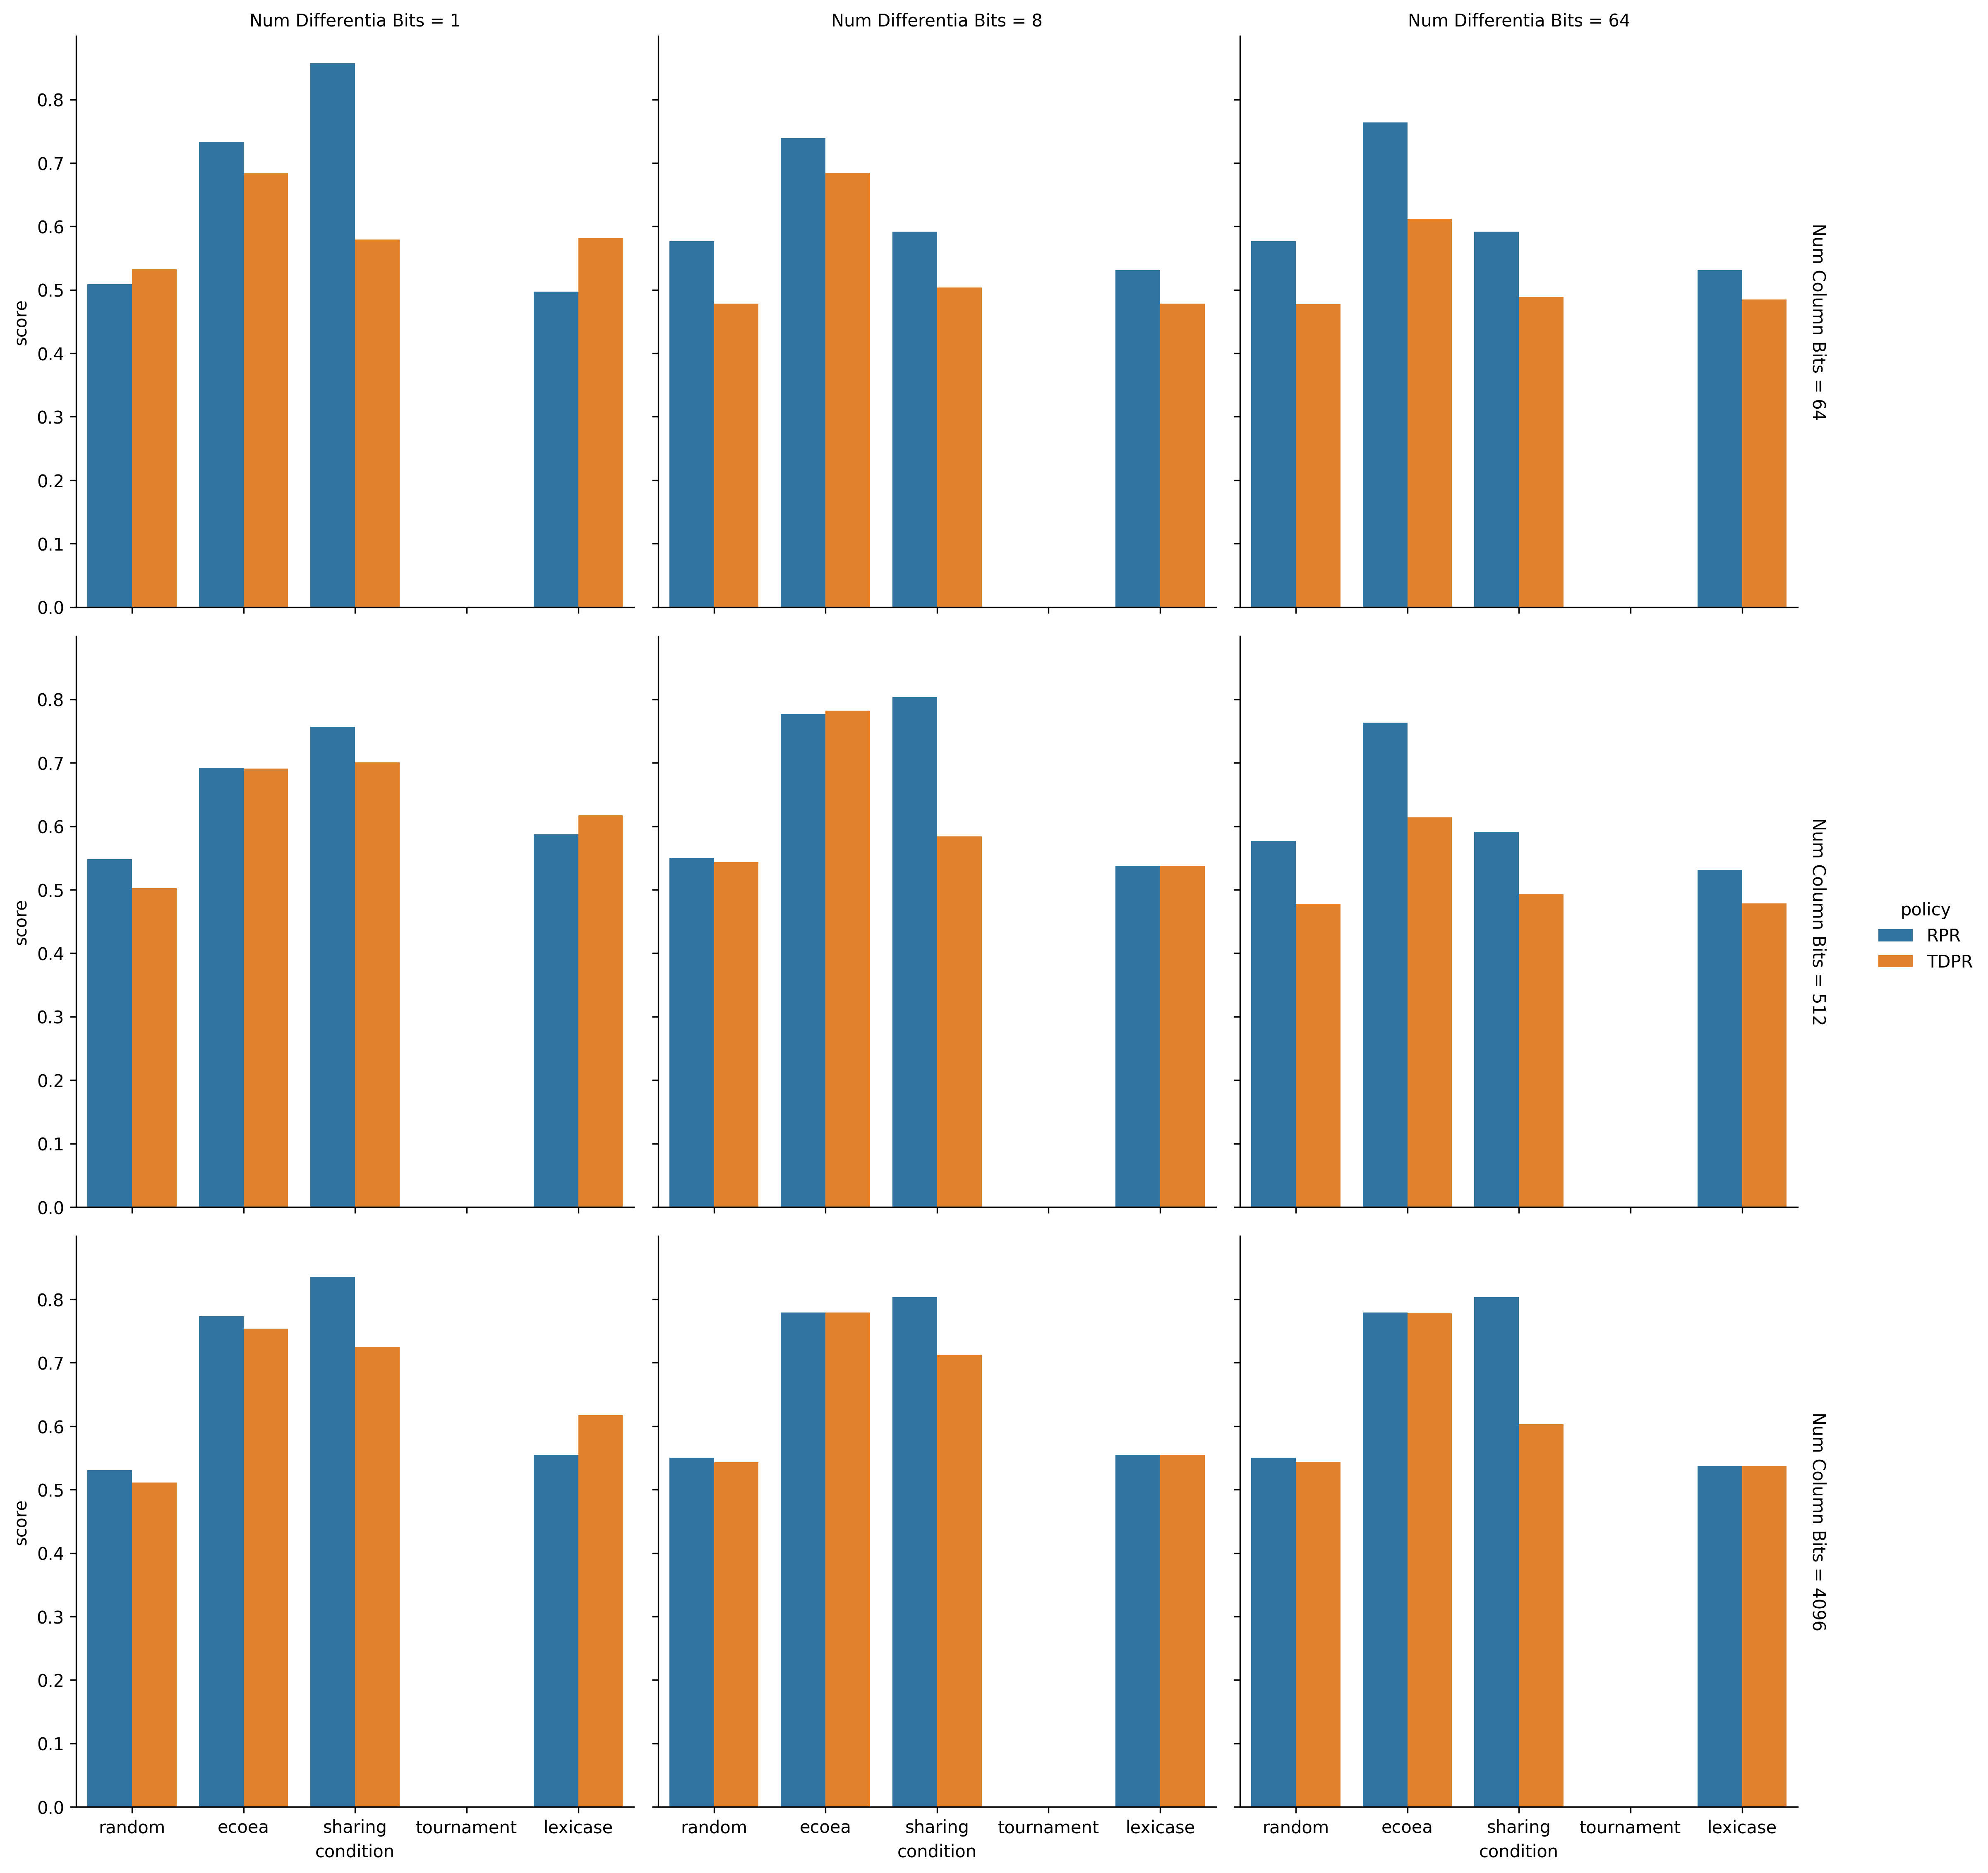
\includegraphics[width=\linewidth]{submodules/hereditary-stratigraph-concept/binder/reconstruction-quality/teeplots/col=num-differentia-bits+hue=policy+kind=bar+row=num-column-bits+tree-comparison-metric=mutual-clustering-information+viz=catplot+x=condition+y=score+ext=}
  \end{minipage}%
  \begin{minipage}{0.3\linewidth}
    \caption{
    Comparison of phylogenetic reconstruction quality between stratum retention policies.
    Reconstruction quality measured as mutual clustering information between reconstructed phylogeny and ground truth phylogeny \citep{smith2020information, smith2020treedist}.
    Higher is better.
    RPR is recency-proportional resolution stratum retention policy and TDPR is tapered depth-proportional resolution stratum retention policy.
    }
    \label{fig:diffbits-mutual-clustering-information}
  \end{minipage}
\end{sidewaysfigure}
